% Tempo di dimezzamento
\newcommand{\tmez}{t_{1/2}}

%\part*{Lezione 04/03/2021}
\subsection{Teoria di Fermi}\label{sec-teofermi}
Ci concentriamo sulla teoria elaborata da Fermi riguardo al decadimento $\beta$.\\
Innanzitutto, consideriamo la \textbf{regola d'oro di Fermi}\index{regola d'oro di Fermi}, definito $\lambda$ il rate di decadimento:
$$\lambda = \frac{2\pi}{\hbar} |V_{fi}|^2 \rho(E_f)$$
dove $\rho(E_f)$ è la densità degli stati finali\footnote{A volte si trova scritta come $\rho(E_f)=dn/dE_f$.} e $V_{fi} = \int d\Omega \;\psi^*_f V \psi_i$ è l'elemento di matrice\footnote{Abbiamo definito $d\Omega$ come l'elemento di volume differenziale.} dell'interazione responsabile del decadimento.\\
Fermi intuì che fosse necessario introdurre un operatore Lorentz-invariante come osservabile; questo operatore $O_X$ può essere un vettore ($_V$), un assiale ($_A$), uno scalare ($_S$), uno pseudoscalare ($_P$) o un tensore ($_T$) e dev'essere l'esperimento a determinarlo. Oggi sappiamo essere un vettore-assiale, tuttavia nella nostra descrizione lo lasceremo indeterminato.\\ 
Esplicitiamo allora le funzioni d'onda:
$$V_{fi} = g \int [\phi^*_f \phi^*_e \phi^*_\nu] O_X \phi_i d\Omega$$
dove abbiamo indicato con $g$ la \textbf{costante di accoppiamento debole} o \textbf{costante di Fermi}\index{costante di accoppiamento debole@costante di accoppiamento debole $g$}\index{costante di Fermi@costante di Fermi $G_F$}. Introduciamo la notazione per i quadrimpulsi finali $p_e\equiv p $, $p_\nu \equiv q$ e $P_Y \equiv P_f$ e scriviamo i differenziali delle densità di particella:
$$\frac{dn}{dE_f} = \frac{dn_edn_\nu dn_f}{dE_f}$$
\begin{displaymath}
\begin{aligned}
&dn_e = p^2 dp d\hat{p} \frac{\Omega}{h^3} \\
&dn_\nu = q^2 dq d\hat{q} \frac{\Omega}{h^3} \\
&dn_f = P_f^2 dP_f d\hat{P_f} \frac{\Omega}{h^3} 
\end{aligned}
\end{displaymath}
Queste 3 equazioni non sono però indipendenti perché sono legate dalla conservazione del quadrimpulso ($P_f+p+q =0$), per cui $dP_f$ è univocamente determinato da $p$ e $q$:
$$dn = \frac{p^2 dp d\hat{p}\:q^2dqd\hat{q}\:\Omega^2}{h^6}$$
Per comprendere la relazione dalle direzioni $\hat{p}$ e $\hat{q}$ scriviamo le funzioni d'onda per il neutrino e per l'elettrone. Quella del neutrino essendo questo neutro ci aspettiamo sia un'onda piana $\phi_\nu = \exp{(-i\vec{q}\cdot\vec{r}_\nu/\hbar)}/\sqrt{\Omega}$; per quella dell'elettrone dovremmo considerare l'interazione coulombiana col nucleo, ma momentaneamente la trascuriamo quindi $\phi_e = \exp{(-i\vec{p}\cdot\vec{r}_e/\hbar)}/\sqrt{\Omega}$. A questo punto assumiamo l'ipotesi di Fermi, ovvero che il decadimento avvenga in un sol punto\footnote{In altre parole le particelle sono distribuite secondo $\delta(\vec{r}_\nu - \vec{r}_e)\delta(\vec{r}_e-\vec{r}_i)$ con $\vec{r}_i$ posizione del nucleone, che equivale a dire $r_e=r_\nu=r_i$. Questa ipotesi è stata dimostrata sperimentalmente, grazie all'osservazione dei bosoni $W^\pm$ e $Z$ mediatori dell'interazione debole, che avendo una massa \vir{molto grande} hanno range di azione \vir{molto piccoli}.}, per cui utilizzeremo la sola variabile $\vec{r}$ per indicare la posizione: 
$$\int \frac{1}{\Omega} \phi^*_f e^{i\vec{p}\cdot\vec{r}/\hbar} e^{i\vec{q}\cdot\vec{r}/\hbar} O_X \phi_i d\Omega$$
A questo punto, il $Q$-\textit{value} è dell'ordine del MeV, per cui anche gli impulsi del neutrino e dell'elettrone sono di quell'ordine; inoltre le funzioni d'onda nucleari tendono a zero molto rapidamente per $r>r_{nucleare}$, dunque ci aspettiamo di poter approssimare\footnote{Come vedremo questa approssimazione ha senso solo se $\int \phi^*_f O_X \phi_i \not = 0$.} $\phi_e\sim\phi_\nu\sim 1/\sqrt{\Omega}$. Per dare una stima dell'ordine di grandezza dell'argomento dell'esponenziale\footnote{Prendiamo $p\,c \sim 1$ MeV e un raggio tipico di $r\sim 10$ fm.}:
$$|\frac{\vec{p}\cdot\vec{r}\; c}{\hbar\,c}|\simeq \frac{1\cdot10}{200}=0.05\ll 1$$
Questa approssimazione viene detta \textbf{approssimazione a transizione \textit{permessa}}. Perché l'integrale sia non nullo le funzioni d'onda dei nucleoni devono avere la stessa parità.\\
Riscriviamo allora il rate:
$$\lambda = \frac{2\pi}{\hbar}g^2 \Bigl |\int \phi_f^* O_X \phi_i d\Omega\Bigr |^2 \frac{p^2 dp 4\pi}{h^3}\frac{q^2dq4\pi}{h^3}\frac{1}{dE_f}$$
dove abbiamo integrato su $d\hat{q}$ e $d\hat{p}$. Fissata\footnote{In questi conti usiamo $c=1$.} l'energia dell'elettrone, la variazione dell'energia finale sarà data solo da quella dei neutrini $dE_f = dE_\nu = dq$, da cui\footnote{Sul differenziale del rate vedi \complrif{compl-orofermi}.}:
$$d\lambda = \frac{1}{2\pi^3 \hbar^7}g^2 \Bigl |\int \phi_f^* O_X \phi_i d\Omega\Bigr |^2 p^2 dp\, q^2 $$
Il rate così definito può essere riscritto come il numero di elettroni con impulso tra $p$ e $p+dp$ per l'intervallo infinitesimo $dp$: $d\lambda = N(p)dp \propto p^2 q^2 dp$. Esprimiamo $q$ in funzione dell'energia dell'elettrone tramite il $Q$-\textit{value} (che è fissato): $Q = T_Y + T_e + q \simeq T_e + q$ con $T_e = \sqrt{m_e^2 + p^2}-m_e$, quindi $q \simeq Q-T_e$. Abbiamo allora:
$$N(p) \propto p^2(Q-\sqrt{m_e^2 + p^2}+m_e)^2$$
Esprimendo in funzione dell'energia cinetica dell'elettrone $dT_e = pdp/\sqrt{m_e^2+p^2}$ si ottiene:
$$N(T_e) \propto (Q-T_e)^2 \sqrt{(T_e+m_e)^2-m_e^2}\,(T_e + m_e) $$

\paragraph{Valutazione delle approssimazioni} In Figura \ref{0304_teo} riportiamo gli andamenti attesi per $Q\simeq 2.5$ MeV, mentre in Figura \ref{0304_dati} riportiamo i dati sperimentali. Osserviamo che l'andamento del $\beta^+$ è molto simile a quello atteso, mentre il $\beta^-$ presenta nella zona $T_e\to0$ un disaccordo con la teoria; ciò è dovuto al fatto di aver considerato l'interazione coulombiana dei prodotti col nucleo: per dare una spiegazione un po' na\"{i}f, nel $\beta^+$ si produce un positrone che è allontanato dal nucleo, mentre nel $\beta^-$ viene produotto un elettrone, per il quale l'effetto dell'attrazione nucleare non è più trascurabile quando la sua energia cinetica è \vir{bassa}.

\begin{figure}[h]
    \centering
    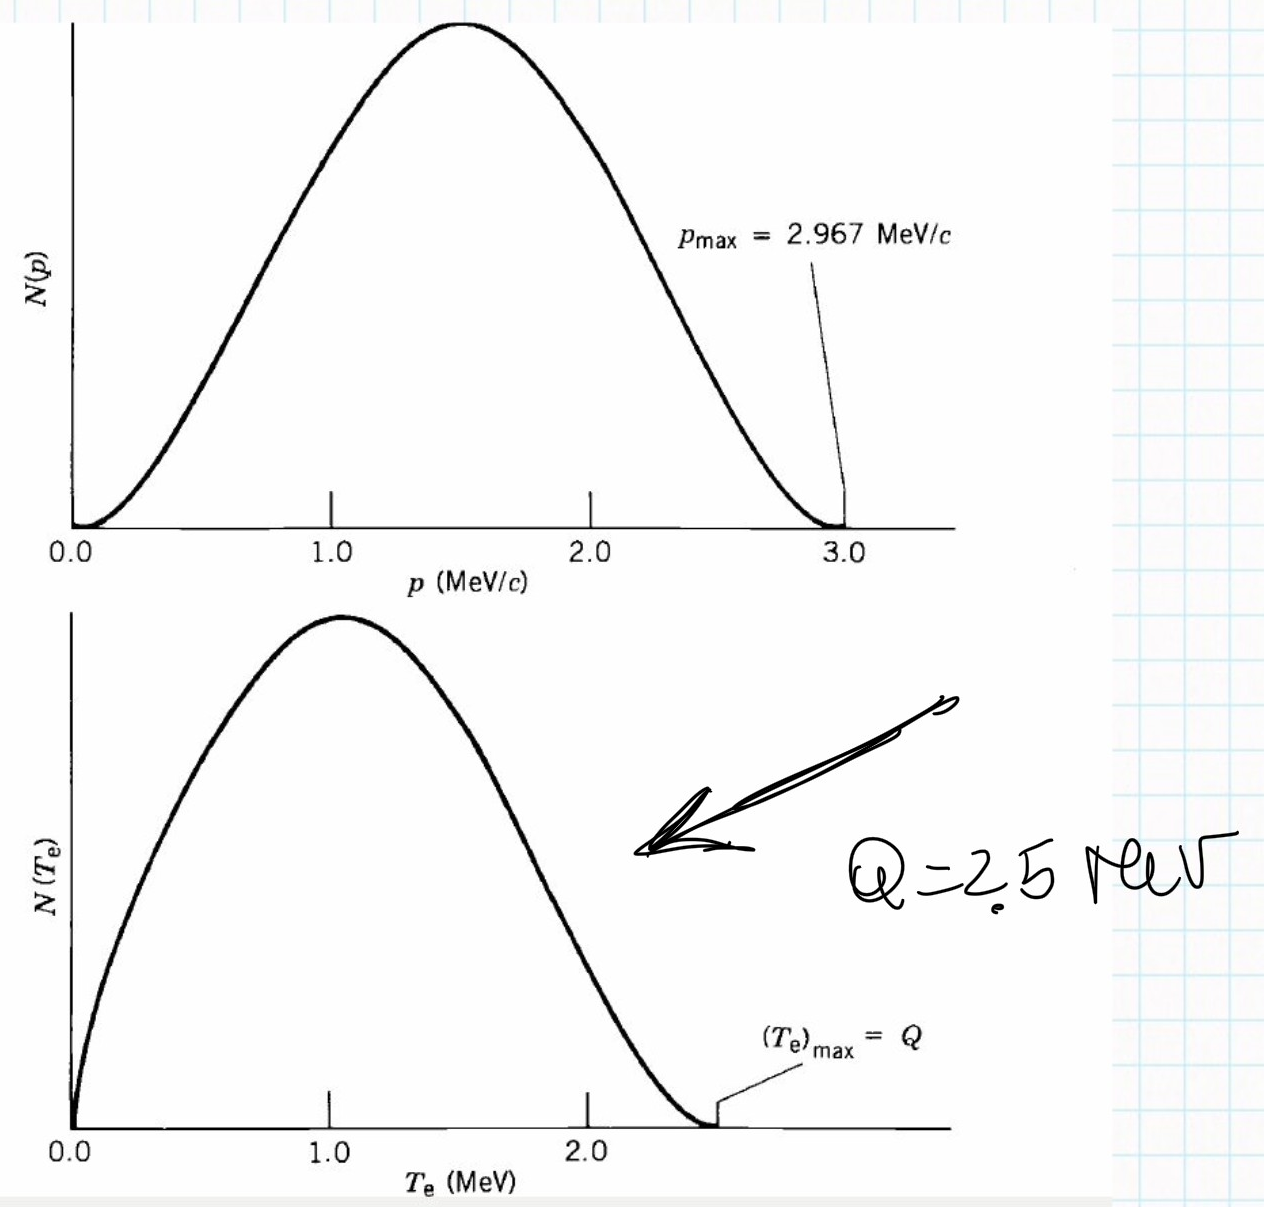
\includegraphics[scale=0.2]{Immagini/0304_andamenti.png}
    \caption{Andamenti teorici del numero di elettroni in funzione dell'impulso (in alto) e dell'energia cinetica (in basso) per il decadimento $\beta$.}
    \label{0304_teo}
\end{figure}
\begin{figure}[h]
    \centering
    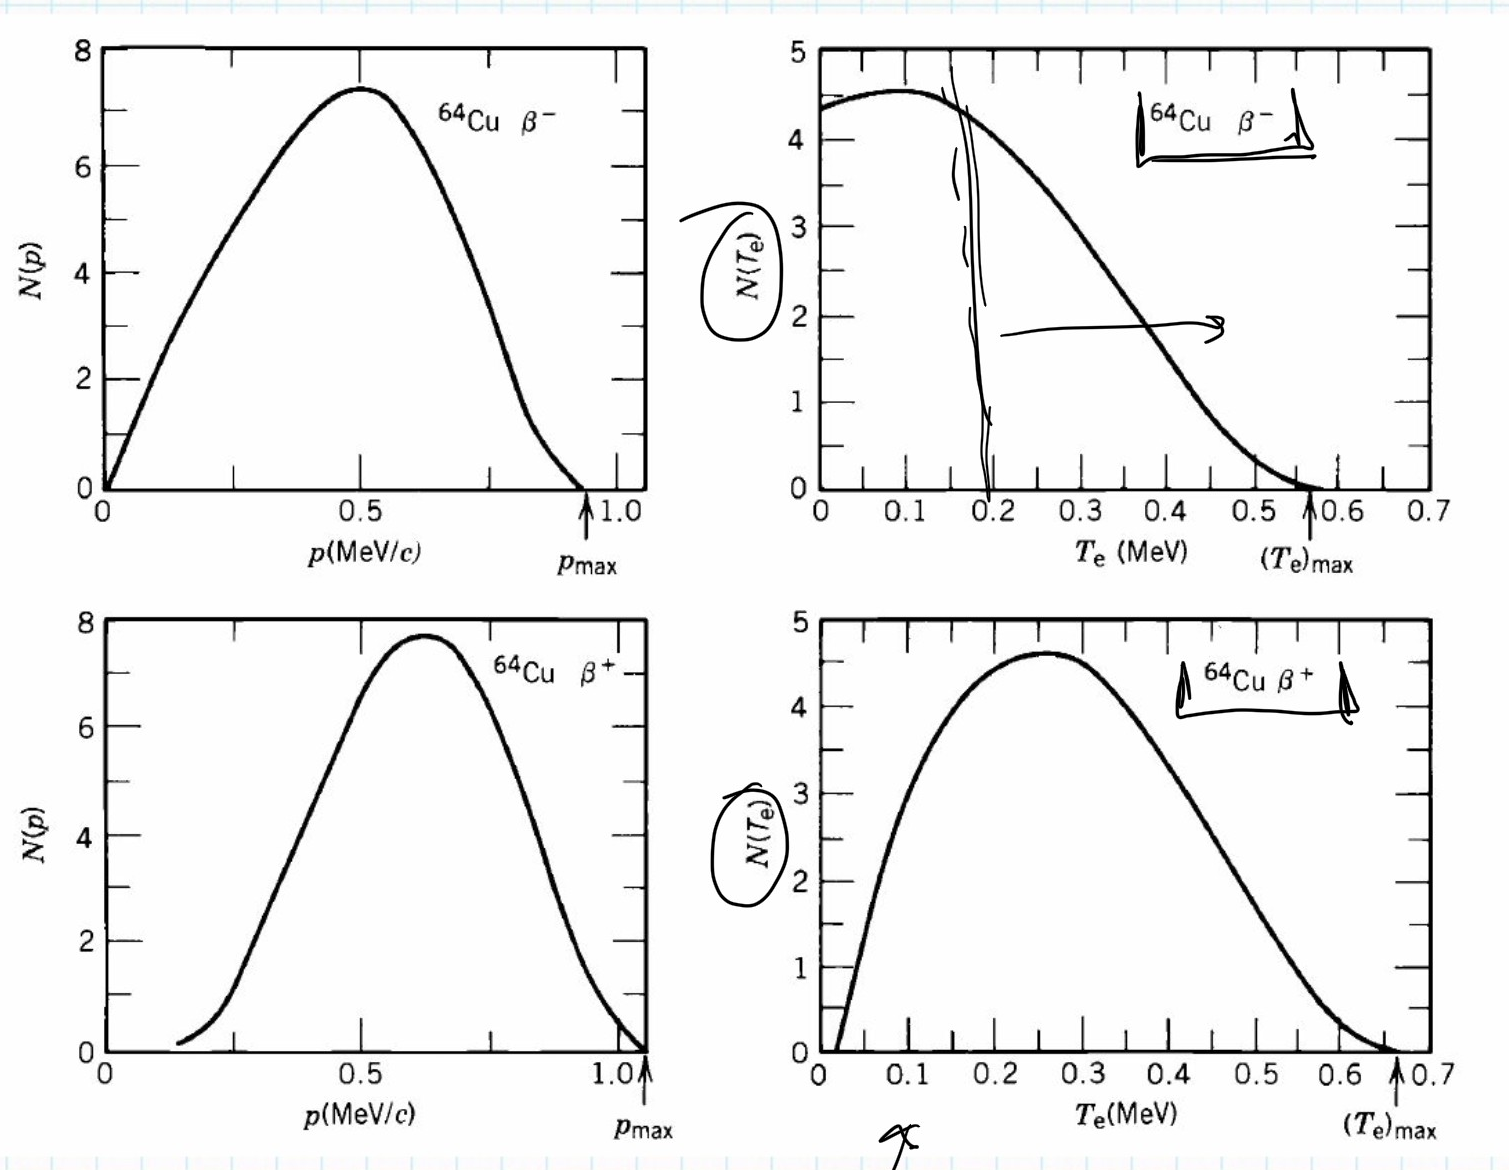
\includegraphics[scale=0.2]{Immagini/0304_andamenti2.png}
    \caption{Dati sperimentali per l'andamento del numero di elettroni nel decadimento $\beta^-$ (in alto) e nel decadimento $\beta^+$ (in basso).}
    \label{0304_dati}
\end{figure}

\noindent Fermi ovviamente aveva chiaro tutto ciò e non utilizzò l'onda piana per rappresentare la funzione d'onda dell'elettrone, ma un'onda distorta. Non riportiamo i calcoli di questa descrizione, ma basti sapere che viene introdotta una fattore correttivo dipendente da $p$ e da $Z_Y$ :
$$N(p)\propto p^2q^2\: F(Z_Y,p)$$
con $F(Z_Y,p)$ \textbf{funzione di Fermi}\index{funzione di Fermi}, che gode della proprietà $F\to 1$ se $p\to\infty$ (alte energie) o $Z_Y\to0$ (carica nulla o trascurabile).\\
Come già anticipato, anche l'approssimazione a transizione \textit{permessa} potrebbe essere non valida, se, per esempio, l'operatore valutato tra gli stati iniziali e finali dei nuclei è nullo, quindi è necessario sviluppare in serie gli esponenziali che compaiono nelle funzioni d'onda del neutrino e dell'elettrone\footnote{Questo comporta che nell'integrazione successiva comparirà una dipendenza dalle direzioni $\hat{p}$ e $\hat{q}$, di cui dovremo tenere conto quando si integra nell'angolo solido.}. Queste transizioni vengono chiamate \textbf{transizioni \textit{proibite}}\footnote{Come avevamo già spiegato, con \textit{proibite} non si intende \vir{non-permesse}, bensì che il tempo di decadimento è molto \vir{lungo} (dal momento che $\lambda$ è minore di quelle \textit{permesse}) e quindi l'osservazione è particolarmente difficile e rara.} e prendono il nome dall'ordine dell'esponenziale al quale ci si ferma\footnote{Nell'espansione non abbiamo riportato i fattori costanti come $\Omega^{-1/2}$ e $\hbar^{-1}$.}:
$$\phi_\nu^* \simeq \underbrace{1}_\text{permessa}+\underbrace{i\vec{q}\cdot \vec{r}}_\text{I proibita}-\frac{1}{2}\underbrace{(\vec{q}\cdot \vec{r})^2}_\text{II proibita}+\dots$$
Considerando tutte le correzioni abbiamo:
$$N(p)\propto p^2(Q-T_e)^2 F(Z_Y,p)\Bigl |M_{fi}\Bigl |^2 S(p,q)$$
dove abbiamo raccolto i termini risultanti dall'integrazione sull'angolo solido in $S(p,q)$, detto \textbf{shape factor}\index{fattore di forma} (che vale 1 se la transizione è \textit{permessa}).\\
Possiamo allora esprimere $(Q-T_e)^2$ come:
$$(Q-T_e)^2\propto\frac{N(p)}{F(Z_Y,p)p^2 S(p,q)}$$
e rappresentarne la'andamento in funzione dell'energia dell'elettrone. Questo grafico è detto \textbf{grafico di Fermi-Kuree}\index{grafico di Fermi-Kuree} e lo riportiamo per il decadimento $0^+\to0^+$ del $\ce{^{66}Ga}$ (che è un \textit{super-permesso}) in Figura \ref{0304_qvalue}. Possiamo notare che per un certo valore dell'energia non vi è più accordo tra teoria ed esperimento a causa dell'interazione dell'elettrone con sorgenti radioattive.\\
Guardiamo, invece, lo stesso grafico per una transizione \textit{proibita} del $\ce{^{91}Y}$ in Figura \ref{0304_qvalue2} e osserviamo l'accordo tra i dati e il modello senza considerare lo shape factor e con lo shape factor.

\begin{figure}[h]
    \centering
    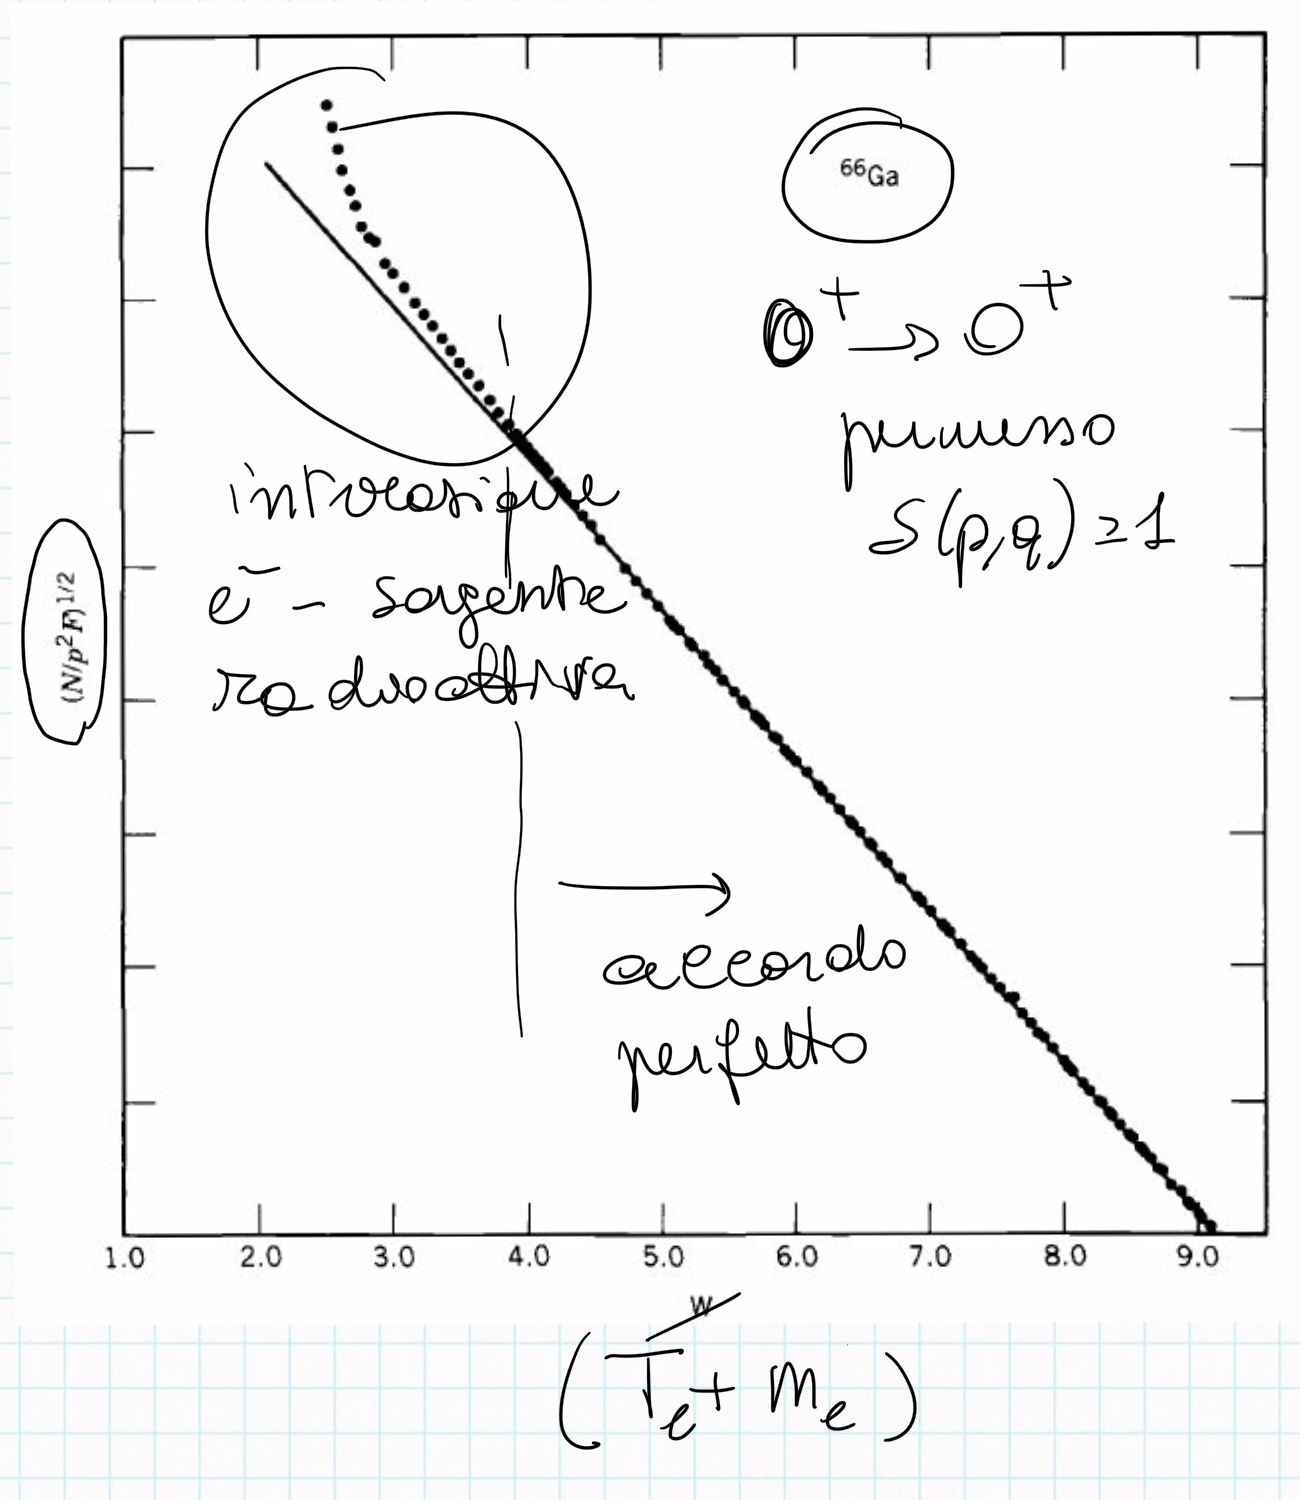
\includegraphics[scale=0.2]{Immagini/0304_andamenti3.png}
    \caption{Grafico di Fermi-Kuree che mostra l'andamento di $(Q-T_e)^2$ in funzione dell'energia dell'elettrone per il decadimento $0^+\to0^+$ del $\ce{^{66}Ga}$ e l'accordo tra i dati e il modello.}
    \label{0304_qvalue}
\end{figure}
\begin{figure}[h]
    \centering
    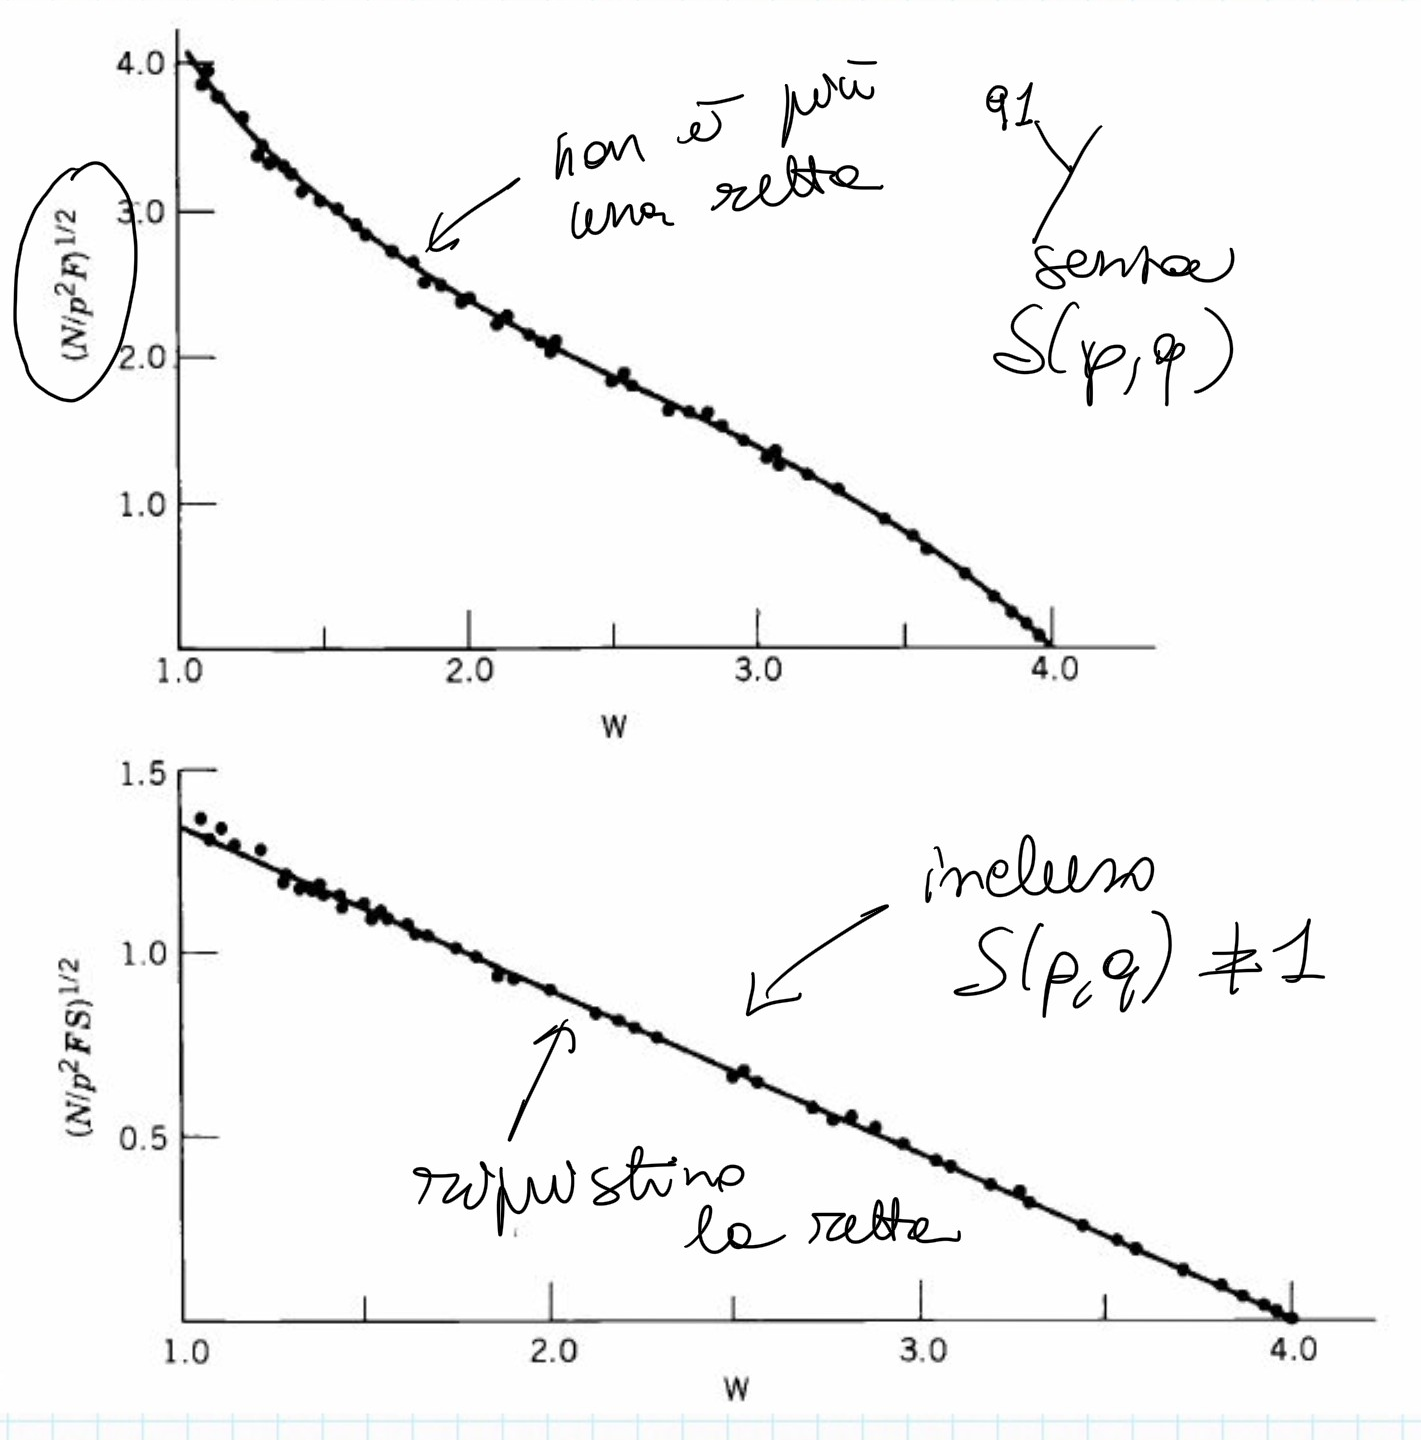
\includegraphics[scale=0.2]{Immagini/0304_andamenti4.png}
    \caption{Grafico di Fermi-Kuree che mostra l'andamento di $(Q-T_e)^2$ in funzione dell'energia dell'elettrone per il decadimento del $\ce{^{91}Y}$ e l'accordo tra i dati e il modello senza shape factor (in alto) e con shape factor (in basso).}
    \label{0304_qvalue2}
\end{figure}

\paragraph{Calcolo del rate} Abbiamo tutti gli strumenti dunque per proseguire con il calcolo del rate\footnote{Per semplicità considereremo un decadimento permesso, ovvero $S(p,q)=1$.}:
$$\lambda = \frac{g^2 |M_{fi}|^2}{2\pi^3 \hbar^7}\int_0^{p_{\max}} p^2 (Q-T_e)^2 F(Z_y,p) dp $$

\begin{definition}[\textbf{Integrale di Fermi}]\index{integrale di Fermi}
$$f(Z_Y,E_0) = \frac{1}{m_e^5 c^5}\int_0^{p_{\max{}}} p^2 F(Z_Y,p)(E_0-E_e)^2 dp$$
dove $E_0\equiv Q + m_e$. Non è un integrale analitico, ma è tabulato per vari $Z_Y$.
\end{definition}
\noindent Per definizione di tempo di dimezzamento $\tmez$ si ha:
\begin{displaymath}
\begin{aligned}
\lambda = \frac{g^2 |M_{fi}|^2}{2\pi^3 \hbar^7} m_e^5\, f(Z_Y,E_0) &= \frac{\ln{2}}{\tmez} \\
f\tmez &= \ln{2}\frac{2\pi^3 \hbar^7}{ g^2 |M_{fi}|^2 m_e^5 c^4} 
\end{aligned}
\end{displaymath}
dove abbiamo inizialmente trascurato $c$ e poi reintrodotta\footnote{$c^{-1}$ compare da $\rho = dn/dE_f = dn/dE_\nu = dn/d(cq)$ che abbiamo calcolato nel paragrafo precedente.}. Quest'ultima espressione viene detta $ft$\textbf{-value}\index{ft-value@$ft$\textbf{-value}} e dipende solo da $|M_{fi}|$ (contributo nucleare), variando in un range esteso, tra $10^3$ e $10^{20}$ s, ragion per cui spesso se ne esprime il logaritmo.\\
Per $\log{(ft)}\sim 3 \div 4$, decadimenti molto veloci, si parla di decadimenti \textit{super-permessi}: sono tutti $0^+\to0^+$ con $M_{fi}\sim \sqrt{2}$ (indipendente dai nuclei in gioco). Questo tipo di decadimento è allora perfetto per stimare la costante di accoppiamento debole $g$ dal momento che presenta per ogni nucleo lo stesso valore $ft$, come riportato in Figura \ref{0304_dati2}; si ottiene così:
$$g\simeq 0.88\cdot 10^{-4} \;\mbox{MeV}\,\mbox{fm}^3$$
Per avere una quantità adimensionale possiamo definire una costante tipica dell'interazione $G = g \,m^2c/\hbar^3$, per cui:
\begin{displaymath}
\begin{aligned}
&\text{Forte } \pi-N & &1 \\
&\text{E.M. } & &10^{-2} \\
&\text{Debole } & &10^{-5} 
\end{aligned}
\end{displaymath}
In quest'ultimo caso viene detta \textbf{costante di Fermi} $G_F$\index{costante di Fermi}.

\begin{figure}
    \centering
    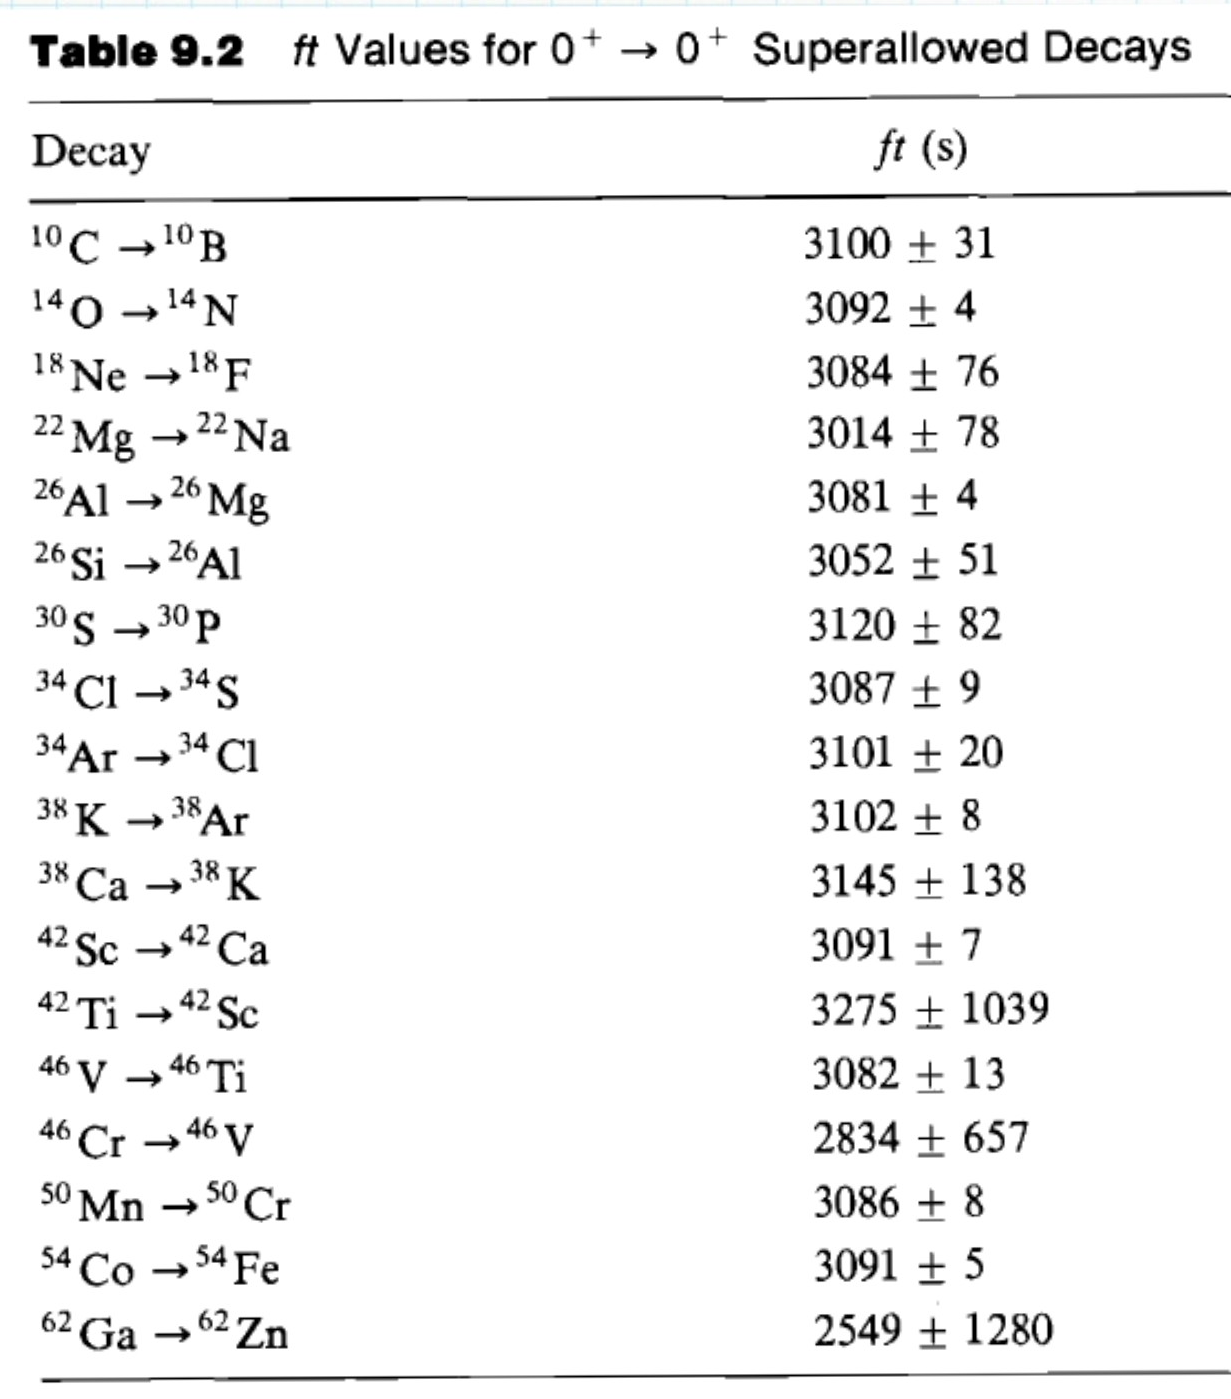
\includegraphics[scale=0.2]{Immagini/0304_dati.png}
    \caption{Tabella con la misura del $ft$-value per il decadimento $0^+\to0^+$ di alcuni nuclei.}
    \label{0304_dati2}
\end{figure}

\subsubsection{La massa del neutrino}\label{sec-nu-mass}
In tutti i calcoli svolti finora abbiamo considerato $m_\nu=0$, ma non è sempre un'approssimazione corretta: per elettroni energetici, ovvero $T_e\to Q$, dalla conservazione dell'energia si ha che $q\ll 1$, quindi il neutrino non è più relativistico ($q\not = Q-T_e$) e gli effetti della sua massa non sono più trascurabili\footnote{Posto $c=1$.} $E_\nu \simeq m_\nu + q^2/2m_\nu$. Poiché ciò influisce sul numero di elettroni, Fermi rielaborò i suoi conti\footnote{Per maggiori dettagli vedi \complrif{compl-neutrini}.} e ottenne un andamento come quello riportato in Figura \ref{0304_nu}.

\begin{figure}[h]
    \centering
    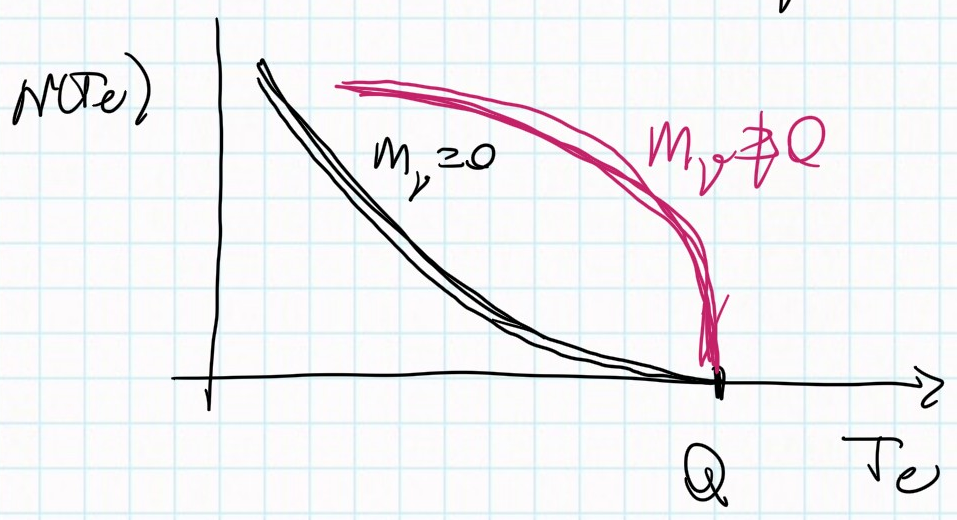
\includegraphics[scale=0.3]{Immagini/0304_neutrini.png}
    \caption{Nel grafico sono rappresentati gli andamenti del numero di elettroni in funzione dell'energia cinetica dell'elettrone senza considerare la massa del neutrino e tenendone conto. Le due curve non sono in scala.}
    \label{0304_nu}
\end{figure}

\paragraph{Esperimenti per $m_\nu$} Ci sono vari esperimenti che cercano di misurare la massa del neutrino; ne discutiamo 2:
\begin{itemize}
    \item \textbf{Katrin}\esperimento{Katrin}: in questo esperimento si sfrutta il decadimento $\beta^-$ del trizio
    $$\ce{^3H}\to\ce{^3He} + e^- +\bar{\nu}_e$$
    In questo modo è possibile misurare direttamente la massa del neutrino, ma proprio per questo è particolarmente difficile.
    \item \textbf{Ptolemy}\esperimento{Ptolemy}: si tratta in realtà di un esperimento ancora in progettazione che prevede di osservare una cattura neutrinica del trizio con neutrini \vir{lenti}.
    $$\nu_e + \ce{^3H}\to\ce{^3He} + e^-$$
    Poiché $T_\nu\sim 0$ l'energia dell'elettrone è fissata (non è più uno spettro continuo) $T_e = m(\ce{^3H}) - m(\ce{^3He}) -m_e +m_\nu $ e dal momento che il trizio decade $\beta^-$ si avrà anche $Q^\beta = m(\ce{^3H})-m(\ce{^3He})-m_e-m_\nu$, da cui\footnote{$m(\ce{^3H}) =Q^\beta -m(\ce{^3He})-m_e-m_\nu$}:
    $$T_e = Q^\beta + 2m_\nu$$
    Ci aspettiamo quindi di osservare un andamento come quello in Figura \ref{0304_nu} dove però compare anche una $\delta$ a distanza $2m_\nu$ da $Q^\beta$. Questa misura permetterebbe quindi di ottenere una stima per $m_\nu$ e un'evidenza sperimentale del \textbf{cosmic neutrino background}, dal quale ci si aspetta neutrini con $T_\nu\sim 0 $.\\
    Questa è, però, anche una della maggiori difficoltà dell'esperimento, ovvero non ci sono ancora state evidenze di questo fondo di neutrini, quindi ci aspettiamo pochissimi eventi; inoltre \vir{immobilizzare} il trizio non è un problema banale: anche se portato a $\sim 0$ K decade molto facilmente $\beta^-$, per cui è stato proposto di legarlo al grafene (o strutture reticolari particolari) in modo da smorzare possibili movimenti.
\end{itemize}

\section{Decadimenti $\beta$ \textit{permessi} e \textit{proibiti}}
Prima di procedere con lo studio di altri decadimenti ci soffermiamo un attimo sulla probabilità di decadimento $\beta$.
\paragraph{Decadimenti permessi} Per questo tipo di decadimenti abbiamo visto che $S(p,q)=1$, da cui $\phi_e\sim\phi_e\sim 1$; $e^\pm$ e $\nu$ sono centrati allora in $r=0$, ovvero non si ha momento angolare orbitale ($\ell = 0$) ma solo \textit{spin} $\vec{S} = \vec{s}_1 + \vec{s}_2$, $S=0,1$:
\begin{displaymath}
\begin{aligned}
S = 1&\,\uparrow\uparrow & &\text{\textbf{Decadimento di Gamow-Teller}}\index{decadimento di!Gamow-Teller} \\
S = 0&\,\downarrow\uparrow & &\text{\textbf{Decadimento di Fermi}}\index{decadimento di!Fermi} 
\end{aligned}
\end{displaymath}
Ci chiediamo quindi quale sia l'operatore $O$ che media il tipo di decadimento. Ci aspettiamo\footnote{Risultati che derivano dalla teoria di campo, che non trattiamo in questa sede.} per il decadimento con $S=0$ di avere uno scalare (1), mentre con $S=1$ un vettore ($\vec{\sigma}$). Per quanto riguarda l'\textit{isospin}, poiché questo passa $-\frac{1}{2} \to \frac{1}{2}$ ($n\to p$) o $\frac{1}{2} \to -\frac{1}{2}$ ($p\to n$)  ci aspettiamo che compaiano gli operatori di salita e discesa dell'\textit{isospin}, ovvero le matrici di Pauli nello spazio dell'\textit{isospin} $\tau^\pm$:
\begin{displaymath}
\begin{aligned}
    \tau^+\st{n}&=\st{p} & \tau^+ \st{\frac{1}{2},-\frac{1}{2}} &=   \st{\frac{1}{2},+\frac{1}{2}}\\
    \tau^-\st{p}&=\st{n} & \tau^- \st{\frac{1}{2},+\frac{1}{2}} &=  \st{\frac{1}{2},-\frac{1}{2}}
\end{aligned}
\end{displaymath}
Riassumendo abbiamo allora:
\begin{displaymath}
O = \Biggl \{
\begin{array}{ll}
    \vec{\sigma}_i \, \tau^\pm_i & S=1\\
     & \\
    1_i \, \tau^\pm_i & S=0 
\end{array}
\end{displaymath}
dove $i$ indica l'$i$-esimo nucleone. \\
Concentriamoci adesso sul momento angolare totale\footnote{Ci riferiamo al momento angolare del nucleo che decade $\vec{J}_i$ che per conservazione è uguale a $\vec{J}_f + \vec{j}$, con $j$ momento angolare dello stato $\nu e^-$. $\Delta J \equiv |\vec{J}_f - \vec{J}_i|$}: poiché questo deve conservarsi si ha per $S=0$ $\Delta J = 0$, mentre per $S=1$ $\Delta J = 0,1$, escluso $J_i=J_f=0$ (per quale si ha invece un decadimento di Fermi). Vediamo alcuni esempi\footnote{Indichiamo con F il decadimento di Fermi e con GT quello di Gamow-Teller}:
\begin{displaymath}
\begin{aligned}
\ce{^{14}O} &\to \ce{^{14}N} & 0^+&\to0^+ & &\text{F} \\
\ce{^{34}Cl} &\to \ce{^{34}S} & 0^+&\to0^+ & &\text{F} \\
n &\to p & \frac{1}{2}^+&\to\frac{1}{2}^+ & &\text{F, GT} \\
\ce{^{6}He} &\to \ce{^{6}Li} & 0^+&\to1^+ & &\text{GT} \\
\ce{^{3}H} &\to \ce{^{3}He} & \frac{1}{2}^+&\to\frac{1}{2}^+ & &\text{F, GT} 
\end{aligned}
\end{displaymath}

\paragraph{Decadimenti proibiti} Non valgono più i decadimenti di Fermi e di Gamow-Teller, perché $\ell\not =0 $, quindi può cambiare la parità ($\pi = (-)^\ell$). Consideriamo $\ell=1$ (I proibito): per $S=0$ $\Delta J = 0,1$\footnote{Questa volta prendiamo entrambi perché si ha un cambio di parità.} e per $S=1$ $\Delta J = 0,1,2$. Alcuni esempi importanti in astrofisica:
\begin{displaymath}
\begin{aligned}
\ce{^{17}N}&\to \ce{^{17}O} & \frac{1}{2}^- &\to \frac{5}{2}^+ & \Delta J = 2 \\
\ce{^{76}Br}&\to \ce{^{76}Se} & 1^- &\to 0^+ & \Delta J = 1
\end{aligned}
\end{displaymath}
Per avere alcuni valori di riferimento:
$$\int \phi_f^* \vec{p}\cdot \vec{r} \phi_i \simeq 0.05 \sim 10^{-2}  $$
$$\lambda \sim |M_{fi}|^2\sim 10^{-4} \lambda_\text{permesso}$$
$$\tau \sim 10^4 \tau_\text{permesso}$$
